\chapter{水下图像合成研究}
海洋包含着未知的生物和巨大能源,对地球上生命延续起着重要的作用。自二十世纪中叶以来,高科技海洋勘测一直备受瞩目,视觉技术因能传达高密度信息而被应用在海洋环境中。研究人员致力于为各种水下应用捕获高质量的水下图像,包括水下机器人、水下救援、生态检测、海洋生物跟踪和实时导航等。

\section{水下图像成像原理及存在问题}
水下环境的特殊物理和化学特性严重影响了水下图像的质量和数量,产生许多比在地面成像的更难克服的问题。如图~\ref{fig:underwater}所示,水下成像存在的问题可以进行详尽分析。

\begin{figure*}[ht]
    \centering
	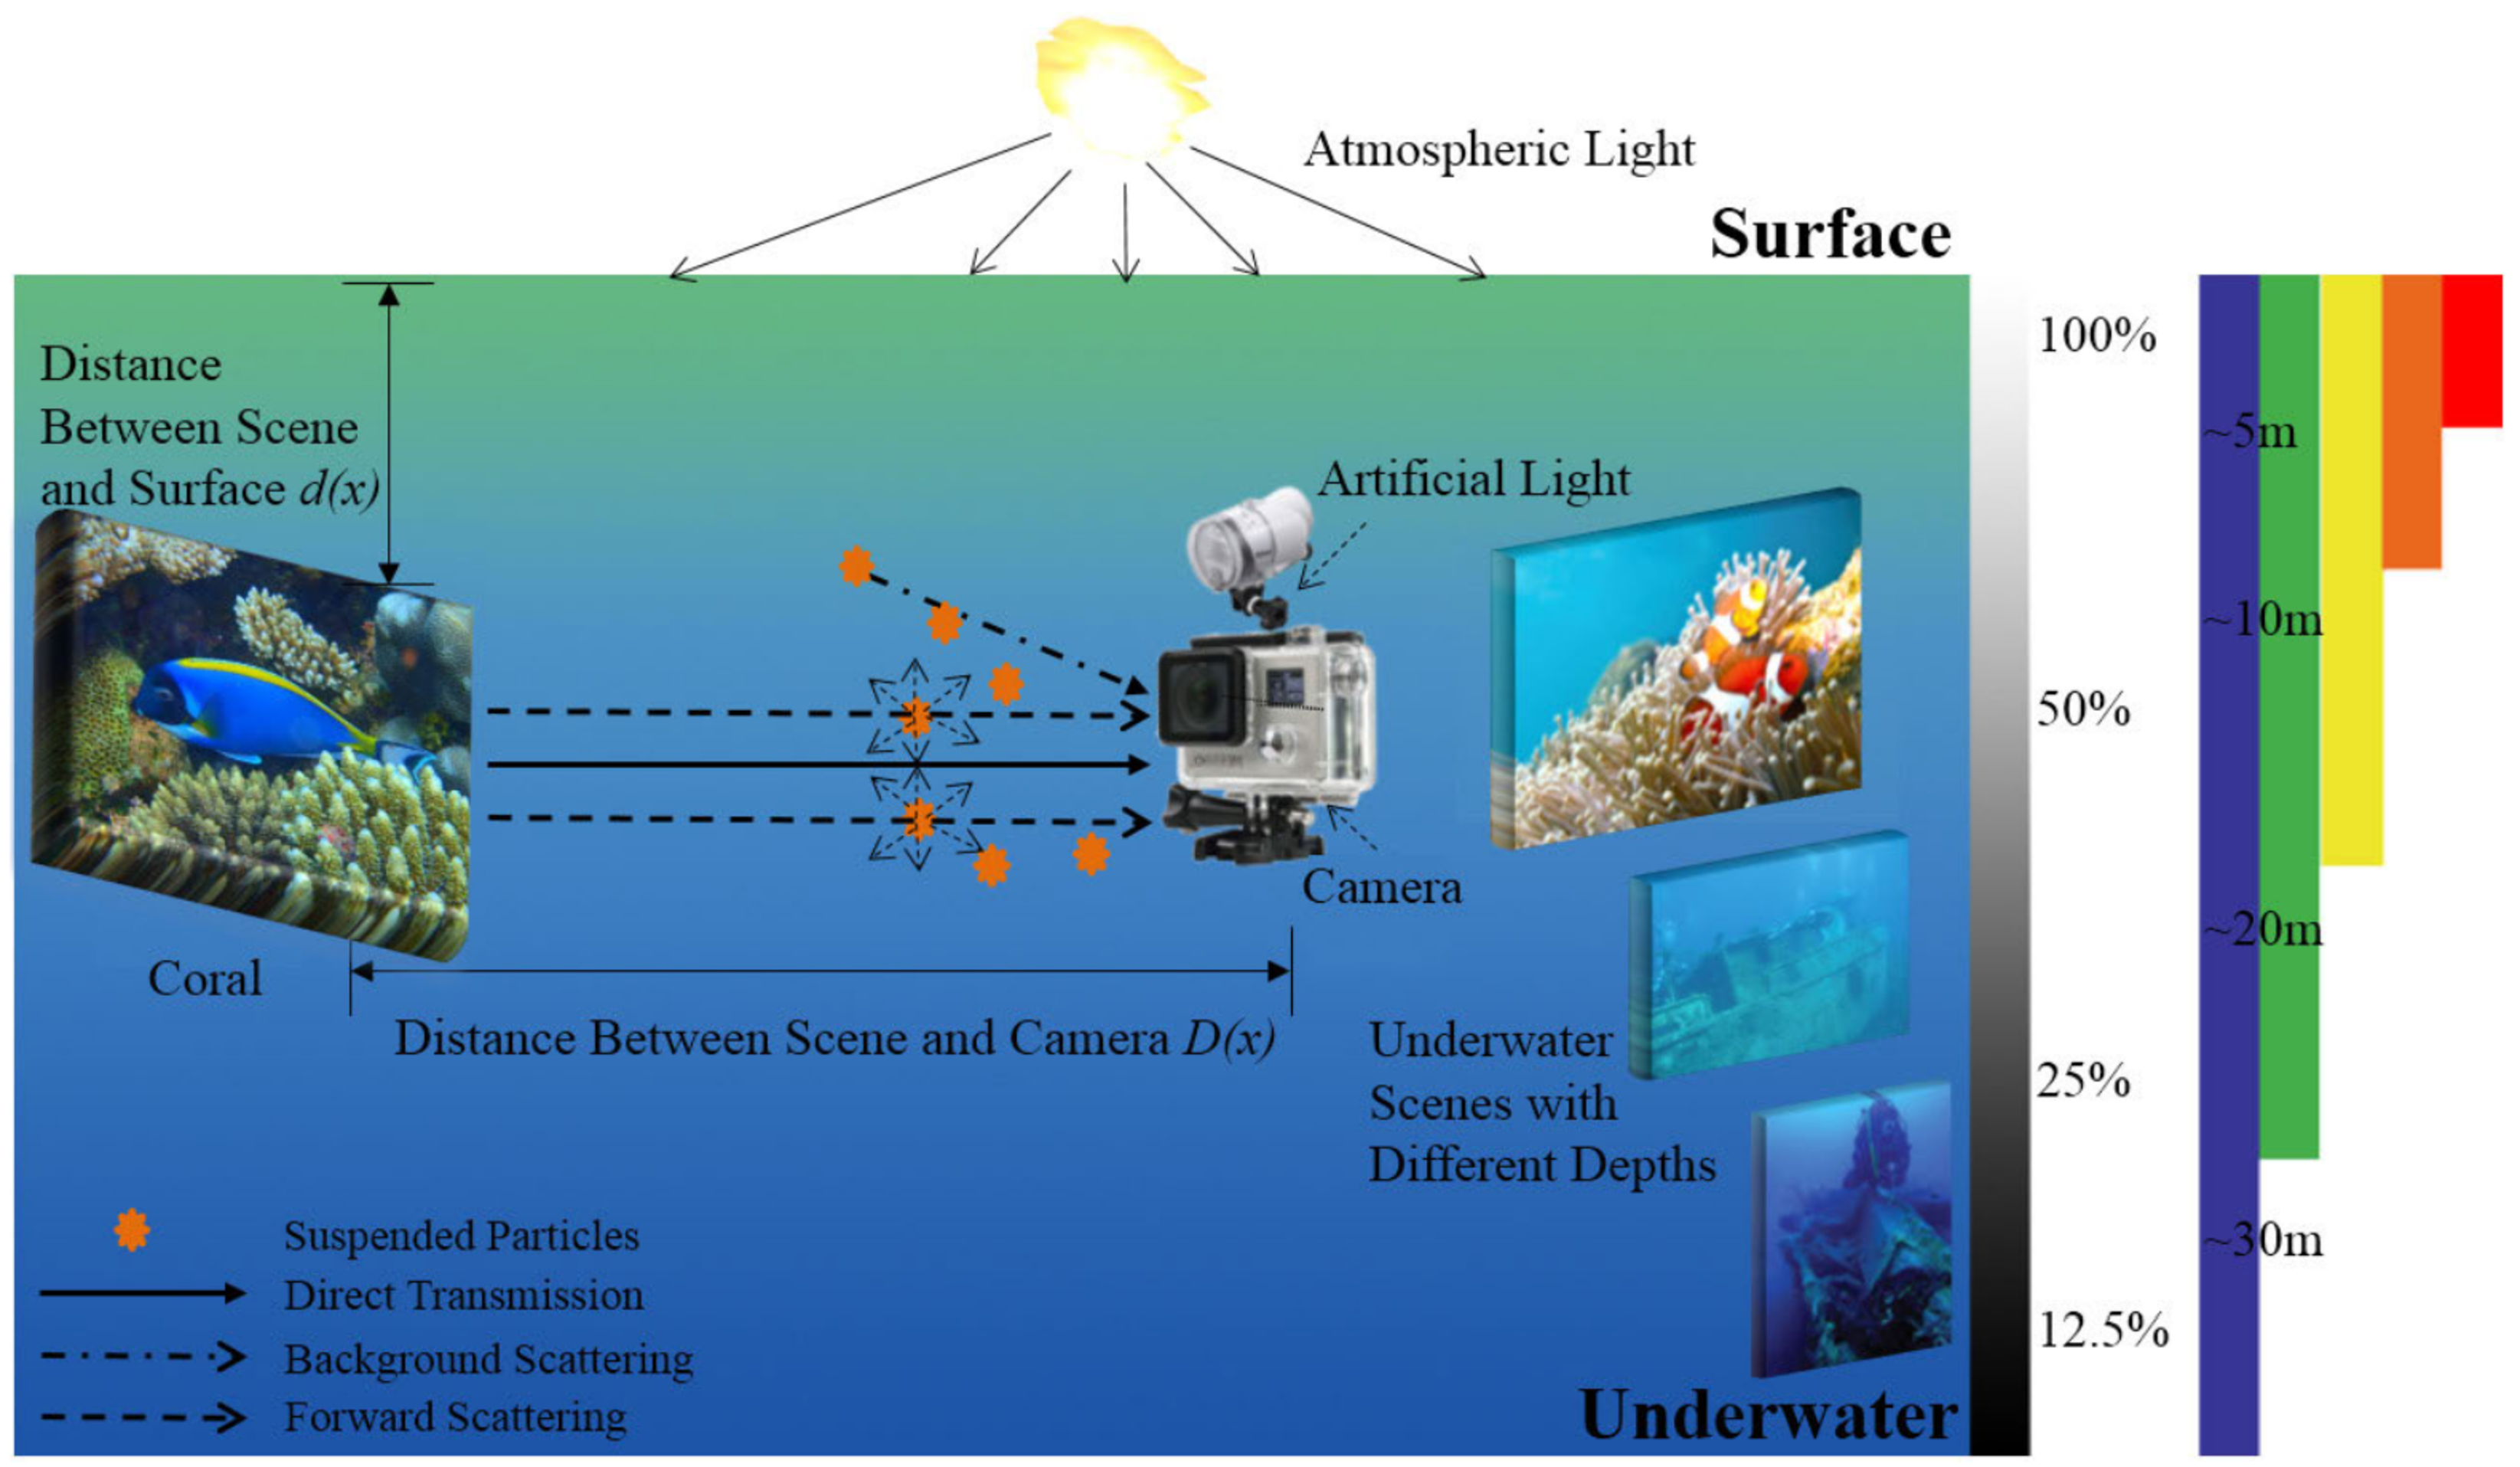
\includegraphics[width=\textwidth]{figs/水下成像.pdf}
	\caption{水下光学成像原理图。}
	\label{fig:underwater}
\end{figure*}

水下图像存在色偏的问题,图像视觉上会呈现蓝色、绿色和蓝绿色。这是由于不同颜色的光在水中的衰减特性造成的,红光波长较长,蓝色和绿色光波长较短,在水介质中光的传播过程中波长较长的光吸收速度更快,因此水下图像呈现蓝绿色调。

水下采集到的图像会存在对比度低,模糊的问题。吸收和散射,即悬浮在水中的颗粒吸收了传播中的大部分光,并将水下场景的反射光在到达相机前改变了光的方向,水的浑浊严重降低了图像质量。人为光线除了吸收和散射,还会出现照明不均匀以及照明不足的问题,会造成阴影。

此外,由于水下环境的成像需要耗费巨大的人力和物力资源,水下图像数据量远远小于非水下自然场景的图像数据量,高质量的图像结果更难能可贵。缺少水下环境中的高质量图像给水下视觉研究造成巨大的困难,这也是研究人员针对水下图像增强和复原进行大量工作的原因。

\section{基于生成对抗网络的水下图像研究}
\subsection{水下图像数据集}
真实水下场景的常用水下数据集数量有限。

UIEB~\cite{anwar2018deep}是具有多样性场景、数量大以及具有高质量参考图像的成对真实场景数据集。原始图像图像共有950张,具有参考图像配对结果的890张,其余60张没有对应的参考图像。采用12种图像增强方法来进行图像增强,针对每张原始图像50个志愿者来选出令人满意的图像增强结果作为真值,令半数以上人不满意的60结果作为挑战图像没有真值。

RUIE~\cite{liu2019real}是共四千多的大规模真实水下数据集。针对可见度增强的性能进行评估的水下图像质量子集,包含五种质量的水下图像其中每种726张,用来测试水下图像增强效果;评估在不同照明和色偏算法的子集,包含蓝色、绿色以及蓝绿色三种色偏的水下图像每种100张;对高级计算机视觉任务如分类和检测的子集,包含对扇贝、海参和海胆三种海洋生物的标注每种100张。

水下图像数据集相比较于非水下场景(空中)图像数量非常少,进行水下视觉图像研究时,研究人员会按照任务需要将空中图像进行水下环境条件模拟。

UWCNN论文中提出的从地面图像得到相应水下图像数据集。通过RGB-D NYU-v2 indoor数据集生成10种类型的水下图像。RGB-D NYU-v2 indoor共1449张图像,其中的1000张用于训练,剩下的449张用于测试,数据集提供的10类水图像也是共1449张图像。对于每张室内图像,根据生成的随机均匀全球大气光和深度(从0.5米到15米,每张图像生成5张水下图像。RGB-D NYU-v2 indoor数据集中的图像作为ground truth(真图),和合成的水下图像(假图)配对。

EUVP是UGAN~\cite{fabbri2018enhancing}中提出数据集的基础上更加齐全的数据集。UGAN中,ground truth是真实的相对不失真的水下图像(真图),配对的是生成的失真的水下图像(假图)。从ImageNet中选择一些不失真的水下图像,组成X域,共6143张图像,再从ImageNet中选择一些有明显水下图像特点的水下图像,组成Y域,共1817张图像。用CycleGAN实现风格迁移,即将X域中不失真的图像转成Y域中失真水下图像的风格(主要是颜色的变化)。最终用于训练的图像对是将X域中的图像都转译成失真水下图像。EUVP中,分为paired和unpaired两种。Paired文件夹中包含3个子文件夹:Underwater Dark、Underwater ImageNet和Underwater Scenes,其中Underwater Dark有5550个图像对,570张验证图像,共11670张;Underwater ImageNet有3700个图像对,1270个验证图像,共8670张图像;Underwater Scenes有2185个图像对,130个验证图像,共4500张图像。Unpaired:poor quality中有3195张,good quality中有3140张,validation中有330张,共6665张图像。

SUN数据集共包含908个类别和131067张图像,用其中采样良好的397个类别去评估场景识别算法。水下图像只是其中一类,一些论文中会用到SUN数据集去做水下增强和复原。仅关注水下图像,有5类:coral reef、ocean deep、ocean shallow、pool、wreck。

\subsection{水下图像评价指标}
UCIQE~\cite{yang2015underwater}和UIQM~\cite{panetta2015human}是无参考/无真值评价水下图像质量的常用指标,在图像增强和图像复原任务中被广泛应用。

\begin{equation}
\label{equ:uciqe}
UCIQE = c_1 \times \sigma_c + c_2 \times con_l + c_3 \times \mu_s
\end{equation}

UCIQM是色彩浓度,饱和度和对比度为测量分量的线性组合,可以定量的评价水下增强结果的色偏、模糊和对比度情况。属于无参考/无真值的图像质量评价指标,首先将水下图像从RGB颜色空间转换到CIELab颜色空间,这样更符合人类视觉感知,然后计算个测量分量,具体计算如式~\ref{equ:uciqe}所示。其中,$ \sigma_c$为色度的标准方差,$con_l$为亮度的对比度,$\mu_s$是饱和度的平均值,$c_1$,$c_2$和$c_3$分别为线性组合的权重值。

\begin{equation}
\label{equ:uiqm}
UIQM = c_1 \times UICM + c_2 \times UISM + c_3 \times UIConM
\end{equation}

UIQM针对水下图像的退化机理和成像特点,采用色彩测量UICM,清晰度测量UISM和对比度测量UIConM作为评价水下图像质量的依据。UIQM属于无参考/无真值的图像评价指标,通过测量分量的线性组合来表征图像的视觉质量,如式~\ref{equ:uiqm}所示。其中,$c_1$,$c_2$和$c_3$分别为线性组合的权重值,权重值的设定需要视具体任务而定,评价水下图像的颜色偏差修正结果时,需设定色度测量分量UICM更大的权重因子;当评价对比度和清晰度时,需要设定清晰度测量分量UISM和对比度测量分量UIConM更大的权重因子。

尽管,两种无参考的指标一定程度上给出定量的图像评价分数,但缺点也很明显。首先,水下图像质量不佳的视觉类型较多,仅参考几个测量分量的线性组合对于图像评价是片面的,缺少客观性和准确性;其次,测量分量权重的设置具有主观性,难以公正的评价水下图像质量;最后,评价结果域视觉效果不一致,会出现指标指示评价较好但视觉上没有直观的展现图像的优越性。


\subsection{经典水下图像合成方法}
目前现有基于生成对抗网络的水下图像处理模型,大多是利用海洋光学成像原理/无监督图像转译方法将空中图像转译成相对应的成对水下图像,目的都是为图像增强和图像恢复提供配对图像数据,图像处理模型训练有监督的网络结构实现图像增强/图像恢复。代表性的工作如下,

UWCNN~\cite{anwar2018deep}是一种基于卷积神经网络的经典图像增强模型。在NYU v2~\cite{Silberman:ECCV12}深度数据集上,将海洋光学成像原理利用深度图应用于合成十种不同类型的水下图像,针对每种水下矮图像类型分别训练多个UWCNN模型,能够模拟各种退化的水下图像以进行水下数据增强。训练集使用NYU v2数据集合成配对的十种类型水样,测试集选择网络上的水下真实图像测试训练好的每种水样类型的UWCNN效果。

UGAN~\cite{fabbri2018enhancing}使用CycleGAN来生成水下图像,从而为进行颜色矫正提供数据。在整个过程中,需要在水下和陆地两个单独的域中拍摄物体图像。使用生成对抗网络作为生成模型,构造将水下图像的真实外观估计变成成对图像转译问题,使用来自两个域的图像作为输入和真值。使用ImageNet的子集来训练和评估网络性能。UGAN-P是在UGAN基础上加入梯度差异损失,直接惩罚生成器中图像梯度预测的差异来增强预测。

WaterGAN~\cite{li2017watergan}提出无监督的水下图像色彩矫正模型。RGB-D的地面图像数据集和水下图像样本集作为输入使用WaterGAN合成与RGB-D对齐的相应水下结果,用生成的水下结果和地面结果作为配对数据训练图像复原模,测试使用真实的水下图像,输出矫正后的图像和相对深度图。

UWGAN~\cite{wang2019uwgan}将彩色RGB图像及其深度图作为输入,然后通过生成对抗性训练学习参数,从而基于水下光学成像模型合成不同类型的水下真实图像。提出用于水下图像恢复和增强的U-net体系结构,比较了U-net中不同损失函数的影响,在此基础上提出了最适合水下图像恢复的损失函数。

Underwater-GAN~\cite{yu2018underwater}基于生成对抗网络,将Wasserstein GAN与梯度惩罚项作为基本网络框架的图像复原模型,对抗损失和感知损失作为生成器损失。恢复水下图像由于复杂的水下成像环境和恶劣的光照条件而产生的退化。数据集不存在成对的清晰图像以及相应的退化水下图像,从网上收集3000张清晰图像作为真值,使用清晰图像来模拟17中不同衰减进行训练和测试。

% Multiscale dense GAN是一种水下图像增强模型,解决原始水下图像的色彩失真、曝光不足和模糊问题。生成器中提供了MSDB(residual multiscale dense block),其中的multiscale, dense concatenation, 和residual learning可以分别提高性能,渲染更多细节并利用残余信息的功能。

Uplavikar等提出水下增强模型~\cite{uplavikar2019all},问题是水类型的多样性使得难以用一个模型来完美实现全部水类型的增强,该工作提出一个Encoder-Decoder卷积网络结构,将不同水类型视为不同域消除相应干扰来学习图像的内容特征。将NYU v2深度数据集合成10种Jerlov风格水样~\cite{anwar2018deep}作为训练数据,UIEB作为测试数据。%如图~\ref{fig:all_in_one}所示,
Encoder将图像编码到潜在空间时,还进行了水样类型判别,帮助Decoder重建出不带水样类型的增强图像结果。

% \begin{figure*}[ht]
%     \centering
% 	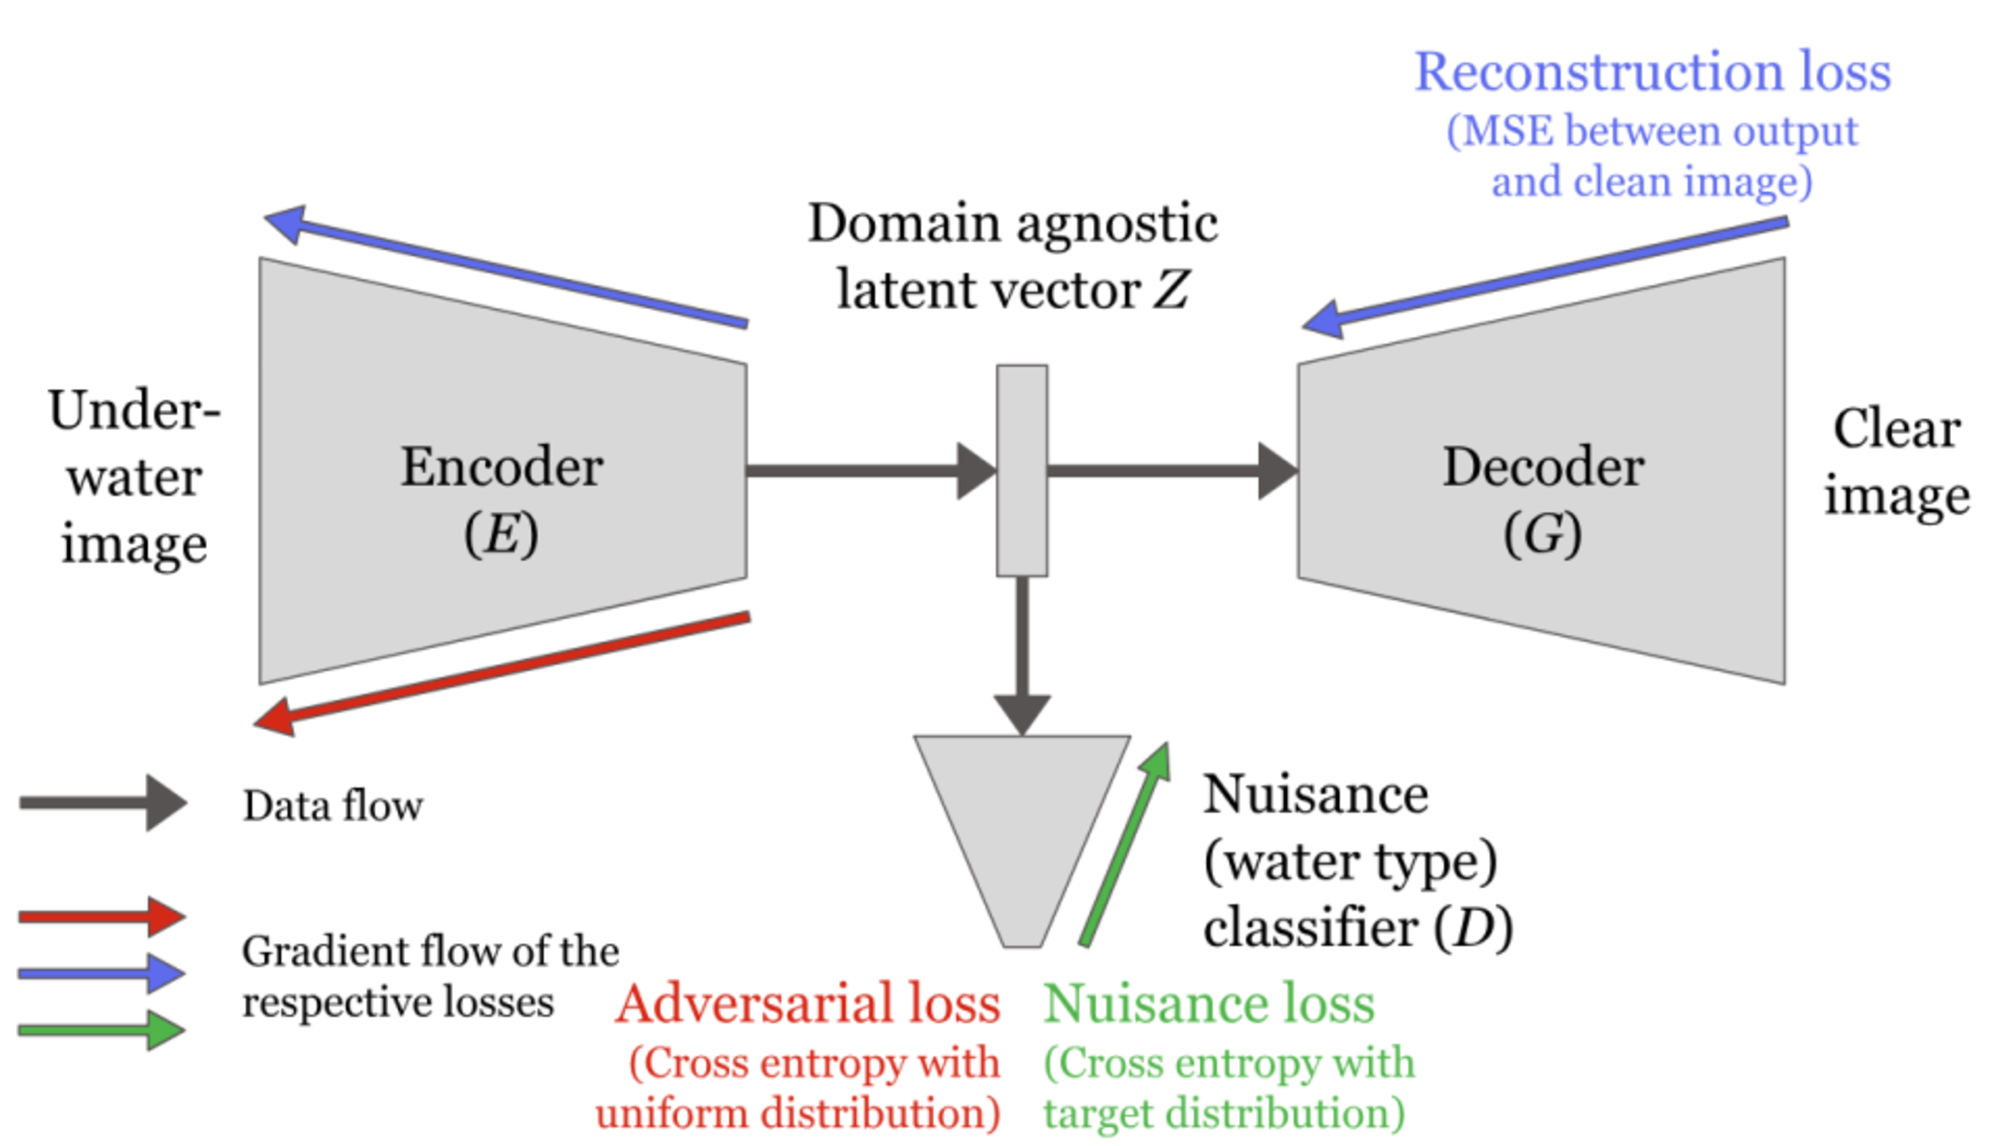
\includegraphics[width=\textwidth]{figs/all_in_one.pdf}
% 	\caption{All-in-One Underwater Image Enhancement Using Domain-Adversarial Learning网络结构图。}
% 	\label{fig:all_in_one}
% \end{figure*}

在进行图像增强和图像复原工作中,往往需要成对的数据,在有监督的网络结构中进行训练,因此水下图像合成方法主要是为了后续研究提供成对的合成数据结果。在上述提到的水下图像合成方法中,主要分成两种类型的合成。一种是利于水下光学成像原理,利用深度图或者传输图作为水下条件将空中图像模拟合成相对应的水下场景图像,如WaterGAN,UWCNN,UWGAN,Underwater-GAN和Uplavikar提出的方法。依赖这种方法始终无法摆脱物理模型的控制,需要深度图/传输图作为指引;且生成水下图像类型固定,若要生成多样化结果需要训练多个模型依次对应。另一种是利用无监督一对一映射的图像转译方法CycleGAN,使用不成对的数据即可进行水下图像合成,如UGAN和MLFcGAN。

这些基于深度学习的水下图像增强和水下图像复原模型,训练需要成对的地面和水下数据进行训练。在缺少成对地面和水下真实数据集情况下,需要使用RGB地面真实图像和深度图/传输图利用海洋光学原理模拟生成不同类型的水下图像结果。这样的方法始终无法摆脱物理模型的控制,需要深度图/传输图作为指引;且生成水下图像类型固定,若要生成多样化结果需要训练多个模型依次对应。
% 其他方法基于深度学习模型,需要深度图等参考生成
% 我们的方法纯正无监督,用生成对抗网络模型直接生成,不用物理设计

\section{基于分解的水下图像研究}


\section{本章小结}
本章主要对水下图像进行研究,为后续研究水下图像转译提供理论基础和数据支撑。

第一小节,介绍了水下图像的成像原理和存在问题。这是现有水下图像增强和水下图像复原任务的出发点和解决目标。

第二小节,对水下任务中常用数据集进行简要介绍,对水下图像评价指标进行研究和分析其原理和合理性,最后是介绍水下图像处理常用的经典方法。


\chapter{水下图像多模态转译模型设计}
本章主要介绍水下图像多模态转译问题以及相应的改进算法。

\section{水下图像多模态转译问题定义}



\section{水下图像多模态转译问题分析}


基于上述几章的分析,我们了解到水下图像合成的方法,一种是基于水下光学物理模型将给定图像合成水下场景图像,另一种是利用CycleGAN这种无监督图像转译模型,实现图像从当前场景到水下场景的转译。

这些问题给水下图像转译问题带来巨大的困难。将有限的给定输入图像,转译成多种水下环境条件的图像结果就显得尤为重要。我们将这种给定图像转译到多种水下环境的图像转译称作水下图像多模态转译。基于生成对抗网络,我们的网络结构可以在无监督条件下,实现水下图像的多模态转译

定义、选择的baselines与问题之间的关系
\section{建立模型算法和损失函数}
\subsection{模型创新点}
\subsection{目标函数和算法}
\subsection{网络结构}
% \section{实验与分析}
% \subsection{数据集设置与实验环境}
% \subsection{评价指标}
% \subsection{消融实验}
% \subsection{与先进方法对比}

\begin{table}[htb]
  \centering\small
  \caption{RUIE数据集上多模态转译定量结果对比}
  \label{tab:ruie_metric}
  \begin{tabular}{l|cccc}
    \toprule
    Metrics & CycleGAN & MUNIT & DRIT & Ours               \\
    \midrule
    FID$\uparrow$     & 243.4 & 139.4 & 179.2 & 0 \\ %textbf加粗
    LPIPS$\downarrow$ & 0.634 & 0.452 & 0.575 & 0 \\
    \bottomrule
  \end{tabular}
\end{table}

\begin{table}[htb]
  \centering\small
  
  \caption{UWCNN数据集上多模态转译定量结果对比}
  \label{tab:uwcnn_metric}
  \begin{tabular}{l|cccc}
    \toprule
    Metrics & CycleGAN & MUNIT & DRIT & Ours               \\
    \midrule
    FID$\uparrow$     & 80.7  & 232.1 & 290.7 & 0 \\ %textbf加粗
    LPIPS$\downarrow$ & 0.490 & 0.647 & 0.668 & 0 \\
    \bottomrule
  \end{tabular}
\end{table}


\section{本章小结}
